% =========================================================
% 3.10.4 দুটি অর্ধযোগক দিয়ে পূর্ণযোগক
% =========================================================

\subsection{দুটি অর্ধযোগক দিয়ে পূর্ণযোগক
(\textenglish{Full Adder Using Two Half Adders})}

আমরা জানি, \textenglish{Full Adder}-এ তিনটি ইনপুট থাকে— \(A\), \(B\) এবং \(C_i\)।
এদের যোগফল নির্ণয়ের জন্য দুটি \textenglish{Half Adder} এবং একটি \textenglish{OR Gate}
ব্যবহার করা যায়। এই পদ্ধতিটি খুবই গুরুত্বপূর্ণ, কারণ এর মাধ্যমে বোঝা যায়
কীভাবে একটি তুলনামূলক জটিল সার্কিটকে সহজ সার্কিটের সমন্বয়ে গঠন করা সম্ভব।

\subsubsection*{কার্যপ্রণালি
(\textenglish{Working Principle})}

প্রথম \textenglish{Half Adder}-এ \(A\) ও \(B\) ইনপুট দেওয়া হয়।

তাহলে প্রথম \textenglish{Half Adder} থেকে পাই—

\[
S_1=A\oplus B
\]

এবং,

\[
C_1=AB
\]

এরপর দ্বিতীয় \textenglish{Half Adder}-এ প্রথম \textenglish{Half Adder}-এর
যোগফল \(S_1\) এবং তৃতীয় ইনপুট \(C_i\) দেওয়া হয়।

তাহলে দ্বিতীয় \textenglish{Half Adder} থেকে পাই—

\[
S=S_1\oplus C_i
\]

অতএব,

\[
S=(A\oplus B)\oplus C_i
\]

সুতরাং,

\[
\boxed{S=A\oplus B\oplus C_i}
\]

আবার, দ্বিতীয় \textenglish{Half Adder}-এর ক্যারি হবে—

\[
C_2=S_1C_i
\]

এখন \(S_1=A\oplus B\) বসালে পাই—

\[
C_2=(A\oplus B)C_i
\]

এখন পূর্ণযোগকের চূড়ান্ত ক্যারি আউট হবে প্রথম ও দ্বিতীয়
\textenglish{Half Adder}-এর ক্যারির \textenglish{OR}।

অর্থাৎ,

\[
C_o=C_1+C_2
\]

এখন \(C_1=AB\) এবং \(C_2=(A\oplus B)C_i\) বসালে পাই—

\[
C_o=AB+(A\oplus B)C_i
\]

এখন \((A\oplus B)\)-এর মান বসাই—

\[
A\oplus B=\overline{A}B+A\overline{B}
\]

সুতরাং,

\[
C_o=AB+(\overline{A}B+A\overline{B})C_i
\]

\[
=AB+\overline{A}BC_i+A\overline{B}C_i
\]

এখন \textenglish{Boolean Algebra} ব্যবহার করে পূর্ণযোগকের বহুল ব্যবহৃত রূপ পাওয়া যায়—

\[
\boxed{C_o=AB+AC_i+BC_i}
\]

অতএব, দুটি \textenglish{Half Adder} এবং একটি \textenglish{OR Gate}
ব্যবহার করে \textenglish{Full Adder} বাস্তবায়ন করা যায়।

\subsubsection*{সারসংক্ষেপ
(\textenglish{Summary})}

\[
\boxed{S=A\oplus B\oplus C_i}
\]

\[
\boxed{C_o=AB+(A\oplus B)C_i}
\]

এবং সমতুল্যভাবে,

\[
\boxed{C_o=AB+AC_i+BC_i}
\]

\par\begingroup

\textbf{মনে রাখবে:}
দুটি \textenglish{Half Adder} দিয়ে \textenglish{Full Adder} তৈরি করলে
প্রথম \textenglish{Half Adder} \(A\) ও \(B\) যোগ করে,
দ্বিতীয় \textenglish{Half Adder} \(S_1\) ও \(C_i\) যোগ করে,
এবং দুটি ক্যারি \textenglish{OR} করে চূড়ান্ত \(C_o\) পাওয়া যায়।
\par\endgroup


\begin{figure}[!htbp]
    \centering
    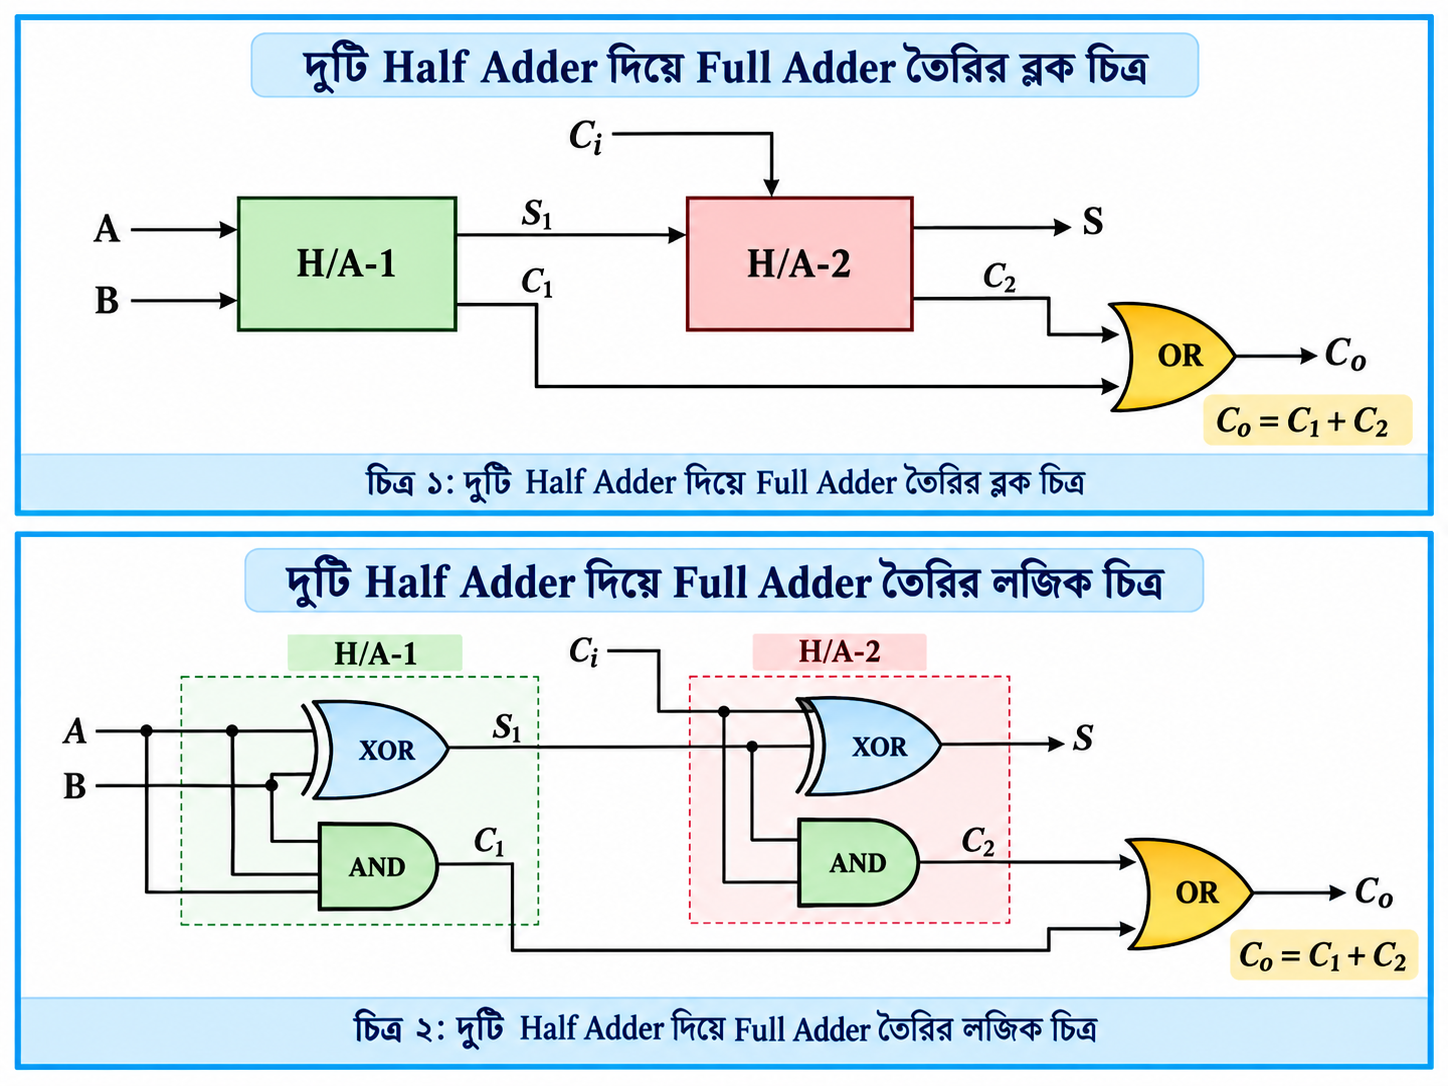
\includegraphics[width=0.92\textwidth]{chapters/Chapter03/resources/images/half_to_full_adder.png}
    \caption*{চিত্র: দুটি \textenglish{Half Adder} এবং একটি \textenglish{OR Gate} ব্যবহার করে \textenglish{Full Adder} বাস্তবায়ন}
\end{figure}


% =========================================================
% 3.10.5 সার্বজনীন গেট দিয়ে পূর্ণযোগক বাস্তবায়ন
% =========================================================

\subsection{সার্বজনীন গেট দিয়ে পূর্ণযোগক বাস্তবায়ন
(\textenglish{Implementation of Full Adder Using Universal Gates})}

আমরা জানি, \textenglish{NAND} ও \textenglish{NOR} গেটকে
সার্বজনীন গেট (\textenglish{Universal Gate}) বলা হয়।
কারণ, এই গেটগুলোর যেকোনো এক ধরনের গেট ব্যবহার করে
যেকোনো \textenglish{Boolean Function} বাস্তবায়ন করা সম্ভব।
সুতরাং \textenglish{Full Adder}-ও শুধু \textenglish{NAND} গেট
অথবা শুধু \textenglish{NOR} গেট ব্যবহার করে তৈরি করা যায়।

\subsubsection*{পূর্ণযোগকের মৌলিক সমীকরণ
(\textenglish{Basic Equations of Full Adder})}

পূর্ণযোগকের তিনটি ইনপুট \(A\), \(B\) ও \(C_i\)-এর জন্য
যোগফল \(S\) এবং ক্যারি আউট \(C_o\) নির্ণয়ের সমীকরণ হলো—

\[
S=A\oplus B\oplus C_i
\]

\[
C_o=AB+AC_i+BC_i
\]

এখন এই সমীকরণগুলোকে এমনভাবে রূপান্তর করা হয়,
যাতে শুধু \textenglish{NAND} বা শুধু \textenglish{NOR} গেট ব্যবহার করে
বাস্তবায়ন করা যায়।

\subsubsection*{\textenglish{NOR} গেট দিয়ে বাস্তবায়নের ধারণা}

\textenglish{NOR} গেট দিয়ে বাস্তবায়নের ক্ষেত্রে
সাধারণত \textenglish{OR} এবং \textenglish{NOT} অপারেশনের উপযোগী রূপে
সমীকরণকে পরিবর্তন করা হয়। \textenglish{De Morgan's Theorem} ব্যবহার করে
বিভিন্ন ধাপে রাশিকে \textenglish{NOR}-উপযোগী আকারে লেখা হয়।
এরপর প্রাপ্ত রাশি অনুযায়ী লজিক সার্কিট আঁকা হয়।

\subsubsection*{\textenglish{NAND} গেট দিয়ে বাস্তবায়নের ধারণা}

\textenglish{NAND} গেট দিয়ে বাস্তবায়নের ক্ষেত্রে
সমীকরণকে এমনভাবে ভেঙে লেখা হয়, যাতে
\textenglish{AND} এবং \textenglish{NOT}-নির্ভর রূপ থেকে
শুধু \textenglish{NAND} গেট ব্যবহার করে আউটপুট তৈরি করা যায়।
এক্ষেত্রেও \textenglish{Boolean Algebra} ও \textenglish{De Morgan's Theorem}
খুব গুরুত্বপূর্ণ ভূমিকা রাখে।

\subsubsection*{কেন এটি গুরুত্বপূর্ণ?}

সার্বজনীন গেট দিয়ে \textenglish{Full Adder} বাস্তবায়ন গুরুত্বপূর্ণ, কারণ—

\begin{enumerate}
    \item একটি নির্দিষ্ট ধরনের গেট ব্যবহার করে সম্পূর্ণ সার্কিট তৈরি করা যায়।
    \item \textenglish{IC} ডিজাইনে একই ধরনের গেট ব্যবহার করলে নকশা সহজ হয়।
    \item সার্কিট বিশ্লেষণ ও বাস্তবায়নের দক্ষতা বাড়ে।
    \item \textenglish{Boolean Algebra} ও \textenglish{Gate Realization}-এর সম্পর্ক স্পষ্ট হয়।
\end{enumerate}

\par\begingroup

\textbf{মনে রাখবে:}
\textenglish{Full Adder} বাস্তবায়নে \textenglish{NAND} ও \textenglish{NOR}—
উভয় ধরনের সার্বজনীন গেটই ব্যবহার করা যায়।
বোর্ড পরীক্ষায় অনেক সময় সমীকরণ এবং সার্কিট—দুটিই চাওয়া হয়।
\par\endgroup


\begin{figure}[!htbp]
    \centering
    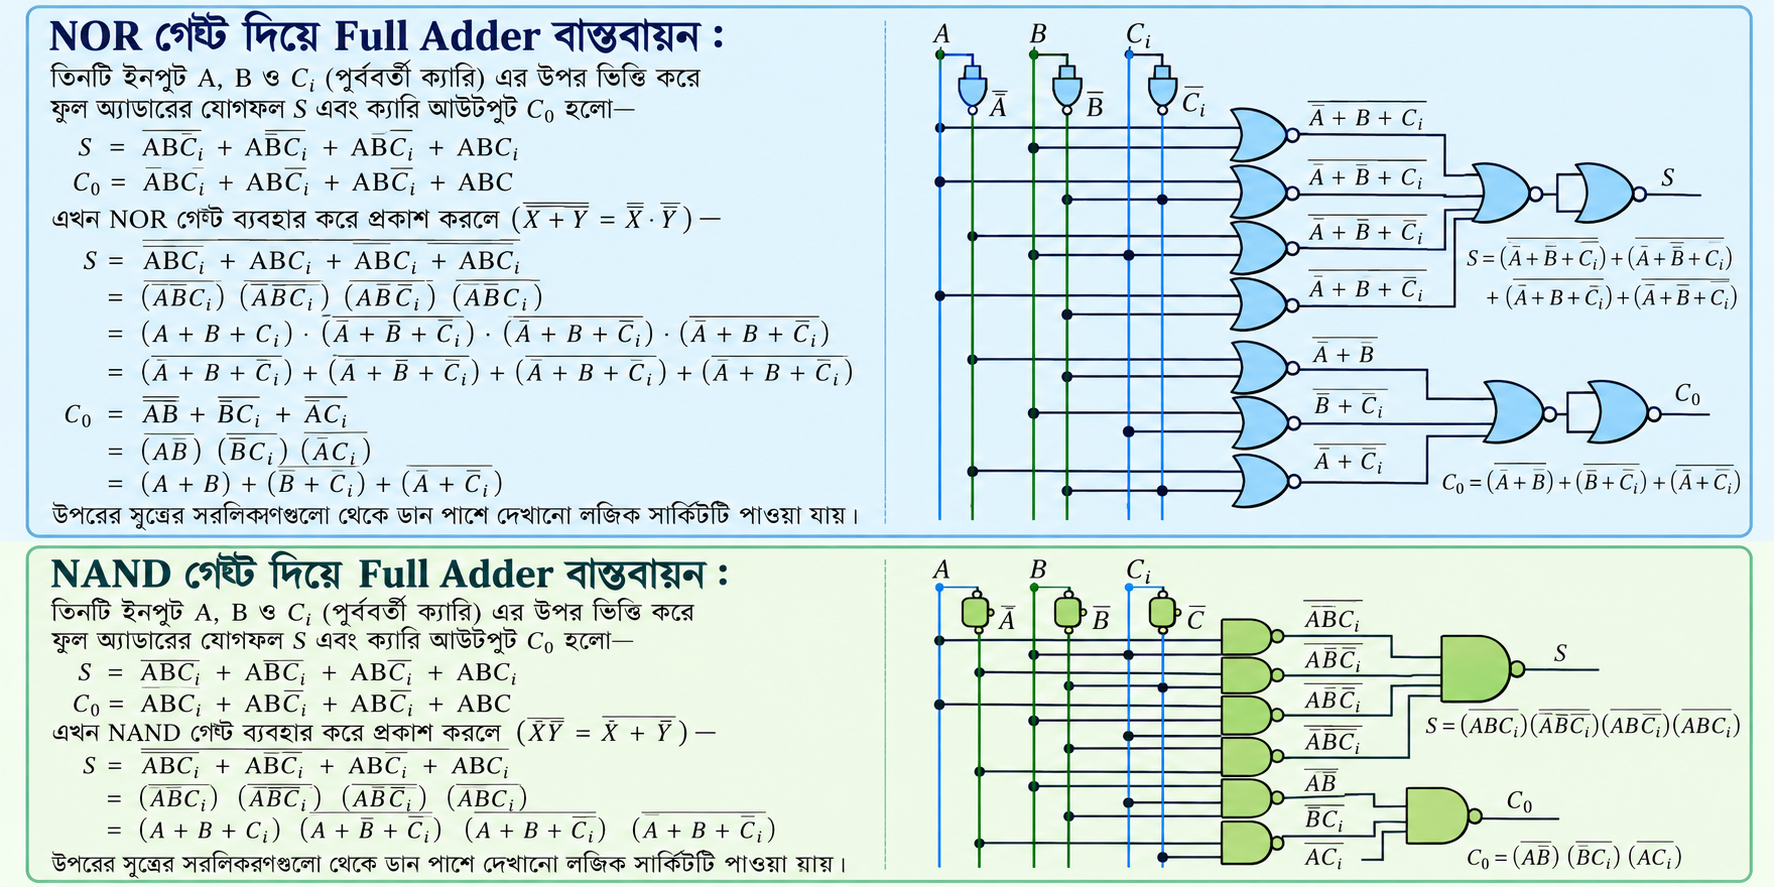
\includegraphics[width=\textwidth]{chapters/Chapter03/resources/images/nand_nor_full_adder.png}
    \caption*{চিত্র: \textenglish{NOR} এবং \textenglish{NAND} গেট ব্যবহার করে \textenglish{Full Adder} বাস্তবায়ন}
\end{figure}

\subsection{নয়টি দুই-ইনপুট গেটে পূর্ণযোগকের ধাপ}
নিচের মধ্যবর্তী সংকেতগুলো অনুসরণ করলে শুধু একই ধরনের গেট দিয়ে যোগফল ও ক্যারি তৈরি করা যায়। $C_i$ ক্যারি ইনপুট এবং $C_o$ ক্যারি আউটপুট।

\smallhead{শুধু NAND}
\[\begin{aligned}
P&=\overline{AB},&Q&=\overline{AP},&R&=\overline{BP},\\
X&=\overline{QR},&U&=\overline{XC_i},&V&=\overline{XU},\\
W&=\overline{C_iU},&S&=\overline{VW},&C_o&=\overline{PU}.
\end{aligned}\]
প্রথম চার গেটে $X=A\oplus B$। পরের চার গেটে $S=X\oplus C_i$। শেষ গেটে $C_o=\overline{\overline{AB}\cdot\overline{XC_i}}=AB+XC_i$। অতএব একই নয় গেটের সংযোগ পূর্ণযোগক।

\smallhead{শুধু NOR}
\[\begin{aligned}
P&=\overline{A+B},&Q&=\overline{A+P},&R&=\overline{B+P},\\
X&=\overline{Q+R},&U&=\overline{X+C_i},&V&=\overline{X+U},\\
W&=\overline{C_i+U},&S&=\overline{V+W},&C_o&=\overline{P+U}.
\end{aligned}\]
প্রথম চার গেটে X হলো A ও B-এর XNOR। পরের চার গেট X ও $C_i$-এর XNOR করলে দুইবার পূরক হয়ে $S=A\oplus B\oplus C_i$ পাওয়া যায়। শেষ NOR-এর ফল $C_o=(A+B)(X+C_i)=AB+AC_i+BC_i$। এখানে X-এর অর্থ NAND নির্মাণের X থেকে আলাদা।

\chThreeExample{১}{দুই half adder-এর মধ্যবর্তী মান}
$A=1,B=0,C_i=1$।
\chThreeAnswer প্রথম half adder-এ $S_1=1,C_1=0$। দ্বিতীয়টিতে $S=S_1\oplus C_i=0,C_2=S_1C_i=1$। শেষ OR-এ $C_o=C_1+C_2=1$। ফল $C_oS=10_2$, যা $1+0+1$-এর সঠিক যোগফল।

\chThreeExample{২}{অ্যাডার দিয়ে বিয়োগ}
চার বিটে $9-5$ নির্ণয় করতে $A=1001$, $B=0101$।
\chThreeAnswer B-এর বিট উল্টে $1010$ এবং প্রথম carry-in ১ দাও।
\[1001+1010+1=1\;0100.\]
অতিরিক্ত ক্যারি বাদ দিলে চার বিটে $0100=4$। এই উদাহরণে A ও B চিহ্নবিহীন মান; চার বিট signed হিসেবে ৯ লেখা যায় না।

